% Created 2024-06-16 Sun 00:13
% Intended LaTeX compiler: pdflatex
ocumentclass[10pt]{article}% =================================BASE====================================%
\documentclass[10pt]{report}
\usepackage[left=2cm,right=2cm,top=2cm,bottom=2cm]{geometry} % Marges
\usepackage[T1]{fontenc} % Nécessaire avec FrenchBabel
\usepackage[utf8]{inputenc} % Important pour symboles Francophones, é,à,etc
\usepackage{csquotes} % Recommandé par PDFLatex lors de la compilation. 


% Calligraphie
%\usepackage{lmodern} % Ça, ça set latin modern
%\usepackage{mathrsfs} %Permet la command \mathscr (Lettres attachées genre) \mathscr(B)

% Calligraphie
%\usepackage{pxfonts} % Met le texte ET les maths en Palatino + donne accès à des symboles math
\usepackage{palatino} % Cette commande met seulement le texte en police palatino
\usepackage{lmodern} % Pour les maths?
% Use lmodern for sans-serif
\usepackage{mathrsfs} % Permet la command \mathscr (Lettres attachées genre) \mathscr(B)





% Bibliographie
%\usepackage[backend=bibtex,style=phys,sorting=ynt]{biblatex}
\usepackage[backend=biber,sorting=ynt,style=ieee]{biblatex}
\addbibresource{/home/charlesedouard/Desktop/Travail/Documentation/master-bibliography.bib}



\usepackage{amsmath, amssymb, amsthm} % Symb. math. (Mathmode+Textmode) + Beaux théorèmes.
\usepackage{mathtools,cancel,xfrac} % Utilisation de boîtes \boxed{} + \cancelto{}{}, xfrac
\usepackage{graphicx, wrapfig} % Géstion des figures.
\usepackage{hyperref} % Permettre l'utilisation d'hyperliens.
\usepackage{color} % Permettre l'utilisation des couleurs.
\usepackage{colortbl} % Color tables
\usepackage[dvipsnames]{xcolor} % Couleurs avancées.
\usepackage{titling} % Donne accès à \theauthor, \thetitle, \thedate

% Physique
\usepackage{physics} % Meilleur package pour physicien. 


% Style
\usepackage{lipsum} % For fun
\usepackage{tikz} % Realisation de figures TIKZ.
\usepackage{empheq} % Boite autour de MULTIPLE équations
\usepackage{bbding}

% Français
\usepackage[french]{babel} % Environnements en Français.
% ==============================BASE-(END)=================================%



% ================================SETTINGS=================================%
% Pas d'indentation en début de paragraphe :
\setlength\parindent{0pt}
\setlength{\parskip}{0.15cm}

% Tableaux/tabular
% Espace vertical dans les tabular/tableaux
\renewcommand{\arraystretch}{1.2}
% Couleur des tableaux/tabular
\rowcolors{2}{violet!5}{}

% Couleurs de hyperliens :
\definecolor{mypink}{RGB}{147, 0, 255}
\hypersetup{colorlinks, 
             filecolor=mypink,
             urlcolor=mypink, 
             citecolor=mypink, 
             linkcolor=mypink, 
             anchorcolor=mypink}


\usepackage{titling} % Donne accès à \theauthor, \thetitle, \thedate

% Physique
\usepackage{physics} % Meilleur package pour physicien. 


% Style
\usepackage{lipsum} % For fun
\usepackage{tikz} % Realisation de figures TIKZ.
\usepackage{empheq} % Boite autour de MULTIPLE équations

% Français
\usepackage[french]{babel} % Environnements en Français.
% ==============================BASE-(END)=================================%





% ================================SETTINGS=================================%
% Pas d'indentation en début de paragraphe :
\setlength\parindent{0pt}
\setlength{\parskip}{0.15cm}

% Tableaux/tabular
% Espace vertical dans les tabular/tableaux
\renewcommand{\arraystretch}{1.2}
% Couleur des tableaux/tabular
\rowcolors{2}{violet!5}{}

% Couleurs de hyperliens :
\definecolor{mypink}{RGB}{147, 0, 255}
\hypersetup{colorlinks, 
             filecolor=mypink,
             urlcolor=mypink, 
             citecolor=mypink, 
             linkcolor=mypink, 
             anchorcolor=mypink}


% Numéros d'équations suivent les sections :
\numberwithin{equation}{section} 

% Les « captions » sont en italique et largeur limitée
\usepackage[textfont = it]{caption} 
\captionsetup[wrapfigure]{margin=0.5cm}

% Retirer l'écriture en gras dans la table des matières
\usepackage{tocloft}
\renewcommand{\cftsecfont}{\normalfont}
\renewcommand{\cftsecpagefont}{\normalfont}

% Change bullet style
\usepackage{pifont}
\usepackage{enumitem}
%\setlist[itemize,1]{label=\ding{224}}
\setlist[itemize,1]{label=\ding{239}}
\renewcommand{\boxtimes}{\blacksquare}
% ================================SETTINGS=================================%



% ==============================NEWCOMMANDS================================%

% Vecteurs de base :
\newcommand{\nvf}{\vb{\hat{n}}}
\newcommand{\ivf}{\vb{\hat{i}}}
\newcommand{\jvf}{\vb{\hat{j}}}
\newcommand{\kvf}{\vb{\hat{k}}}
\newcommand{\uu}{\vb{u}}
\newcommand{\vv}{\vb{v}}
\newcommand{\ust}{\vb{u}_{\ast}}

% Physics empty spaces 
\newcommand{\typical}{\vphantom{A}}
\newcommand{\tall}{\vphantom{A^{x^x}_p}}
\newcommand{\grande}{\vphantom{\frac{1}{xx}}}
\newcommand{\venti}{\vphantom{\sum_x^x}}
\newcommand{\pt}{\hspace{1pt}} % One horizontal pt space

% Moyenne numérique entre deux points de grilles. 
\newcommand{\xmean}[1]{\overline{#1}^x}
\newcommand{\ymean}[1]{\overline{#1}^y}
\newcommand{\zmean}[1]{\overline{#1}^z}
\newcommand{\xymean}[1]{\overline{#1}^{xy}}

% Tilde over psi
\newcommand{\tpsi}{\tilde{\psi}}
\newcommand{\tphi}{\tilde{\phi}}

% Nota Bene env : (\ding{89})
%\newcommand{\nb}{$\boxed{\text{\footnotesize\EightStarConvex}\pt \mathfrak{N. B.}}$\hspace{4pt}}
\newcommand{\nb}{\underline{{\footnotesize\EightStarConvex}\pt $\mathfrak{N.B.}$\vphantom{p}}\hspace{3pt}}


% Define the nota bene environment
\usepackage{tcolorbox}
\newtcolorbox{notabene}{
     colback=blue!5,
     colframe=black,
     boxrule=0.5pt,
     arc=2pt,
     left=5pt,
     right=5pt,
     top=5pt,
     bottom=5pt,
}


\newcommand{\cmark}{\ding{52}}
\newcommand{\xmark}{\ding{55}}
% ==============================NEWCOMMANDS================================%



% ==============================PAGE-TITRE=================================%
% Titlepage 
\newcommand{\mytitlepage}{
\begin{titlepage}
\begin{center}
{\Huge Contrat Été 2023 \par}
\vspace{2cm}
{\Huge \MakeUppercase{\thetitle} \par}
\vspace{2cm}
RÉALISÉ DANS LE CADRE\\ D'UN PROJET POUR \par
\vspace{2cm}
{\Huge ISMER--UQAR \par}
\vspace{2cm}
{\thedate}
\end{center}
\vfill
Rédaction \\
{\theauthor}\\
\url{charles-edouard.lizotte@uqar.ca}\\
ISMER-UQAR\\
Police d'écriture : \textbf{CMU Serif Roman}
\end{titlepage}
}
% ==============================PAGE-TITRE=================================%



% =================================ENTÊTE==================================%
\usepackage{fancyhdr}
\pagestyle{fancy}
\setlength{\headheight}{13pt}
\renewcommand{\headrulewidth}{0.025pt} % Ligne horizontale en haut

\fancyhead[R]{\textit{\thetitle}}
\fancyhead[L]{\ \thepage}
\fancyfoot[R]{\textit{\theauthor}}
\fancyfoot[L]{}
\fancyfoot[C]{} 
% =================================ENTÊTE==================================%
\author{Charles-Édouard Lizotte}
\date{22/09/2023}
\title{Carnet de bord, Université McGill}
\hypersetup{
 pdfauthor={Charles-Édouard Lizotte},
 pdftitle={Carnet de bord, Université McGill},
 pdfkeywords={},
 pdfsubject={},
 pdfcreator={Emacs 27.1 (Org mode 9.6.7)}, 
 pdflang={French}}
\begin{document}

\mytitlepage
\tableofcontents\newpage

\section{{\bfseries\sffamily TODO} Téléchargement de Wavewatch III -- \textit{<2023-09-18 Mon>}}
\label{sec:org7ce919e}
\subsection{Télécharger et construire le modèle}
\label{sec:org2689416}
Avant tout, un courriel m'avait été envoyé avec un lien pour télécharger le modèle à l'adresse \url{https://polar.ncep.noaa.gov/waves/wavewatch/distribution/} en 2019.
Une fois téléchargée, on peut développer l'archive \textbf{tar} dans un nouveau dossier (ww3 dans notre cas),
\begin{verbatim}
  mkdir ww3
  tar -xvf wwatch3.v5.16.tar.gz -C ww3
  cd ww3
\end{verbatim}
On se retrouve avec une multitude de fichiers \textbf{tar} éparpillés au long du dossier \emph{ww3}. 
Pour développer les multiples archives \textbf{tar} restantes, on utilise le script bash d'installation fournit par l'équipe de Wavewatch,
\begin{verbatim}
  chmod +x install_ww3_tar 
  ./install_ww3_tar 
\end{verbatim}
Tout au long de l'installation, quelques questions seront posées sur les compilateurs désirés. Personnellement, j'utilise les compilateurs \emph{gcc} et \emph{gfortran} par habitude.
Par la suite, on s'assure que tout est en ordre à l'aide du script \emph{w3-setup} cachée dans le dossier \emph{ww3/bin}.
Le script \emph{w3-setup} crée l'environnement Wavewatch contenue dans le dossier courant sous le nom de \emph{wwatch3.env}.
De plus, cette commande nous permet de choisir
\begin{enumerate}
\item le répertoire du dossier \emph{ww3} (\emph{home/charlesedouard/Desktop/Travail/ww3});
\item le fichier de compilation associé à notre compilateur (\emph{ww3/bin/comp.gfortran});
\item ainsi que les \emph{switches} nécessaires à la compilation du modèle (\emph{ww3/bin/switch-lizotte}).
\end{enumerate}
Dans mon cas, j'ai mes propres \emph{switches}, c'est pourquoi -- dans la prochaine commande -- on cite \emph{-s lizotte} en référence au fichier \emph{switch-lizotte}.
Plus d'informations là dessus à venir. 
On peut effectuer cette commande depuis le dossier \emph{ww3},
\begin{verbatim}
  ./bin/w3_setup /home/charlesedouard/Desktop/Travail/ww3 -s lizotte -c gfortran
\end{verbatim}

Comme on utilise NetCDF4, il est impératif de créer deux variables d'environnement, soient \emph{WWATCH3-NETCDF} et \emph{NETCDF-CONFIG}, 
\begin{verbatim}
  export WWATCH3_NETCDF=NC4
  export NETCDF_CONFIG=/usr/lib/x86_64-linux-gnu
\end{verbatim}

\nb Pour trouver le répertoire de NetCDF4, on utilise \textbf{nc-config}, 
\begin{verbatim}
  which nc-config
\end{verbatim}

Il serait pertinent d'ajouter ces variables d'environnement à notre \emph{.bashrc} et d'ajouter ajouter \emph{bin} et \emph{exe} à notre \emph{PATH}.
Donc, dans le fichier \emph{.bashrc}, on ajoute
\begin{verbatim}
  export WWATCH3_NETCDF=NC4
  export NETCDF_CONFIG=/usr/bin/nc-config
  PATH=$PATH:/home/charlesedouard/Desktop/Travail/ww3/bin
  PATH=$PATH:/home/charlesedouard/Desktop/Travail/ww3/exe
  export PATH
\end{verbatim}
Là, nous serions rendus l'étape de la compilation du modèle.
La compilation s'effectue à l'aide de la commande \emph{w3-make}, par contre il faut revenir sur les \emph{switches} du modèle.
J'ai mes propres \emph{switches} qui s'assurent que tout fonctionne bien en sortant de la boîte (\emph{switch-lizotte}).
L'intérieur du fichier se lie comme suit
\begin{verbatim}
  F90 NOGRB NOPA LRB4 NC4 TRKNC SHRD PR3 UQ FLX2 LN1 ST2 NL1 BT0 IC0 IS0
  REF1 DB0 TR0 BS0 XX0 WNT1 WNX0 CRT0 CRX0  O0 O1 O2
\end{verbatim}
Pour vérifier si les \emph{switches} sont bonnes, on prend la commande \emph{sort-switch <switches-file> -r}.
La commande \emph{-h} fonctionne pour avoir de l'aide,
\begin{verbatim}
  sort_switch switch_lizotte -r
\end{verbatim}
Finalement, on appliquer le script \emph{w3-make},
\begin{verbatim}
  w3_make
\end{verbatim}
La commande \emph{w3-make} s'applique aussi sur les sous-routines individuelles de Wavewatch,
\begin{verbatim}
  w3_make ww3_grid ww3_shell <...>
\end{verbatim}
Et tout devrait bien compiler!

\subsection{Débuggage NetCDF et OpenMPI}
\label{sec:org1403389}
À ce point, il est possible que la compilation n'ait pas lieu car bien des librairies NetCDF ne sont toujours pas installées.
Si c'est le cas, on peut sudo-installer la commande \textbf{nc-config} à l'aide de la première commande et NetCDF-fortran à l'aide de la seconde, comme proposé dans une réponse produite sur \href{https://stackoverflow.com/questions/73249935/how-to-install-netcdf-fortran-on-ubuntu}{Stack Overlow}.
\begin{verbatim}
  sudo apt install libnetcdf-dev
  sudo apt install libnetcdff-dev
\end{verbatim}
Pour voir si tout est en ordre, on vérifie la command \textbf{nc-config} à l'aide des commandes
\begin{verbatim}
  nc-config --version
  nc-config --all
\end{verbatim}

Il se peut que la librairie contenant \textbf{mpifort} n'est toujours pas installée sur notre ordinateur.
Il existe beaucoup de moyen de l'installer, mais \textbf{cmake} fait des siennes en cherchant un ancient répertoire MPI qui n'existe plus.
La \href{https://github.com/pytorch/pytorch/issues/33521}{solution} proposée par un utilisateur GitHub est donnée par
\begin{verbatim}
  # sudo apt install openmpi-bin
  # sudo apt-get install mpich
  sudo apt-get install libopenmpi-dev
\end{verbatim}


\section{{\bfseries\sffamily DONE} Faire fonctionner le modèle standard -- \textit{<2023-09-19 Tue>}}
\label{sec:orge78a486}
\begin{wrapfigure}[15]{r}{0.45\textwidth}\vspace{-\baselineskip} \centering \hspace{0.5cm}
\centering
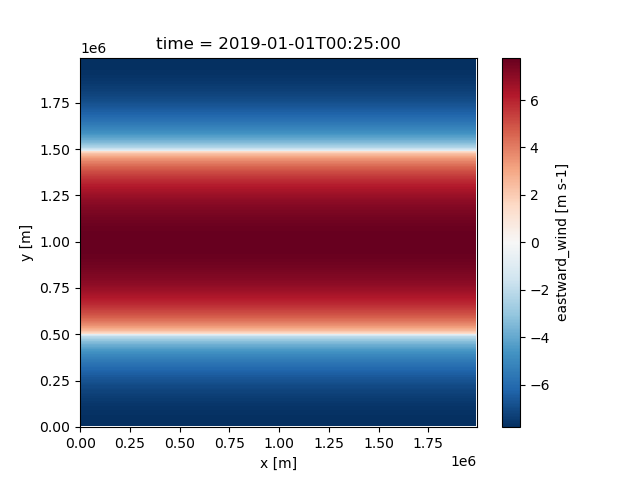
\includegraphics[width=0.35\textwidth]{figures/tests/2023_09_20_east_wind_from_ww3.png}
\caption{\label{fig:org28b20db}Output du vent sorti d'une rapide run de Wavewatch. Les axes sont bien ordonnés donc les input sont réglementaires.}
\end{wrapfigure}


\subsection{Re-Construire la grille, la mapsta et les forçages -- \textit{<2023-09-19 Tue>}}
\label{sec:org8b0dfb9}
\label{orgde4f3db}
Heureusement, j'avais sauvegardé beaucoup de matériel avant l'annihilation de Mingan, dont quelques fonctions Python qui construisent les champs, soient
\begin{itemize}
\item \emph{build-grids.py};
\item \emph{build-current.py};
\item \emph{build-wind.py}.
\end{itemize}
J'en ai aussi profité pour les remetter à jour avec NetCDF4.
Quelques problème d'orientation des variables et dimensions sont apparus.
Il semble que je gérais très mal ce problème lors de maîtrise, mais le code est maintenant béton.
Mentionnons que les NetCDF doivent impérativement avoir des coordonnées dans l'ordre
\begin{itemize}
\item \emph{time} (temps) ;
\item \emph{y} (latitude) ;
\item \emph{x} (longitude).
\end{itemize}
et que cet ordre doit \textbf{aussi} se retrouver dans le vecteur à l'intérieur du NetCDF et/ou du \textbf{xarray.Dataset}.
Après ces efforts, le modèle semble bien rouler sans problème.
Ce mardi le modèle était finalement bien installé avec toutes les librairies nécessaires, aujourd'hui les fonctions produisant les forçages nécessaires au couplage sont créés.
Il ne reste donc qu'à vérifier si le modèle prend tout et après on peut se lancer dans le couplage.\bigskip

Ce mercredi midi, le modèle fonctionne à merveille.

\section{{\bfseries\sffamily DONE} Faire fonctionner le modèle en MPI -- \textit{<2023-09-21 Thu>}}
\label{sec:org2ac1674}
\subsection{Déterminer les bonnes switches pour la compilation MPI -- \textit{<2023-09-20 Wed>}}
\label{sec:org23860c8}
Maintenant que le modèle \emph{standalone} fonctionne efficacement, on doit le lancer en MPI.
Il faudra d'abord changer les \emph{switches}.
Essentiellement, les \emph{switches} permettent au script \textbf{w3 make} de prendre les fichiers \emph{ftn} et et des retirer des lignes de code inutiles.
Ce faisant, le script les transforment en fichiers compilable de type \emph{.o} (objets) et les met dans le dossier \emph{ww3/obj}.
Par la suite, le script de compilation choisi (initialement \emph{comp.gfortran}) transforme ces objets en exécutables qu'on peut retrouver dans le dossier \emph{exe}.
Les \emph{switches} contrôlent donc tout, au final. \bigskip

Ainsi, lors de la compilation standard de Wavewatch 3 (voir section \ref{orgde4f3db}), nous avions actionné les \emph{switches} suivantes : 
\begin{verbatim}
   F90 NOGRB NOPA LRB4 NC4 *SHRD* PR3 UQ FLX2 LN1 ST2 NL1 BT0 DB0 TR0 BS0 IC0 IS0 REF1 XX0 WNT1
   WNX0 CRT0 CRX0 TRKNC O0 O1 O2
\end{verbatim}

Par contre, le \href{https://polar.ncep.noaa.gov/waves/workshop/pdfs/WW3-workshop-exercises-day4-MPI.pdf}{workshop de la NOAA} disponible en ligne insiste modifier deux \emph{switches}, soient \textbf{DIST} et \textbf{MPI} pour remplacer la \emph{switch} \textbf{SHRD}.
Notre fichier de \emph{switches} devrait donc ressembler à
\begin{verbatim}
   F90 NOGRB NOPA LRB4 NC4 *DIST MPI* PR3 UQ FLX2 LN1 ST2 NL1 BT0 DB0 TR0 BS0 IC0 IS0 REF1 XX0
   WNT1 WNX0 CRT0 CRX0 TRKNC O0 O1 O2
\end{verbatim}

\subsection{Compiler le modèle en MPI -- \textit{<2023-09-21 Thu>}}
\label{sec:org5ef9cb0}
Ensuite, il faut le compiler.
Normalement, pour utiliser MPI, on change \textbf{gfortran} par \textbf{mpif90} lors de la compilation.
Par contre, ça ne semble pas marcher du tout.
J'ai testé plusieurs types de compilations, tels que \emph{mpifort} et \emph{mpif90}, ce qui a pris beaucoup de temps.
Après un peu de recherche, il semble que certaines sous-routines de Wavewatch 3 ne voulaient pas être compilées à cause d'une minuscule ligne d'appel MPI en Fortran.
Par exemple, les sous-routines
\begin{itemize}
\item \emph{w3iorsmd.ftn};
\item \emph{w3iosfmd.ftn};
\item \emph{w3waves.ftn}
\end{itemize}
posaient problème.
Mentionnons que la ligne problématique était
\begin{verbatim}
  INCLUDE "mpif.h"
\end{verbatim}
et que la plupart des compilateurs \emph{mpifort} et \emph{gfortran} peuvent avoir de la misère avec ça.
On a donc du se tourner vers un autre compilateur, soit \emph{ifort}. 


\subsection{Installer les compilateurs ifort et mpiifort -- \textit{<2023-09-21 Thu>}}
\label{sec:orgf390f41}

Avant tout, faire ça pour purger les détritus liés à une précédente suite Intel,
\begin{verbatim}
  sudo apt autoremove intel-hpckit
  sudo apt update
\end{verbatim}
Ensuite, on peut utiliser le \href{https://fortran-lang.discourse.group/t/how-to-install-only-a-few-compiler-components-of-the-intel-oneapi-kits-on-ubuntu/3834/4}{script d'un utilisateur d'un forum Fortran} pour installer \emph{ifort}, \emph{icc}, \emph{icpc} et \emph{mpi},
\begin{verbatim}
  sudo apt install \
       intel-oneapi-compiler-dpcpp-cpp-and-cpp-classic \
       intel-oneapi-compiler-fortran \
       intel-oneapi-mpi-devel
\end{verbatim}
Si ça marche pas au final, on peut faire ça, mais c'est 9Go, c'est la \href{https://www.intel.com/content/www/us/en/docs/oneapi/installation-guide-linux/2023-0/apt.html\#APT-PACKAGES}{solution proposée par le site de Intel}. 
En somme, ça installe toute la \href{https://www.intel.com/content/www/us/en/developer/tools/oneapi/toolkits.html\#gs.60r1wa}{suite Intel HPC toolkit}, soit
\begin{verbatim}
  sudo apt install intel-hpckit
\end{verbatim}
Après, il faut ajouter \emph{ifort} et les autres options de compilation au \emph{PATH}, comme proposé dans le \href{https://www.intel.com/content/www/us/en/docs/fortran-compiler/get-started-guide/2022-2/get-started-on-linux.html}{Getting Started on Linux}.
En fait, il serait préférable d'ajouter ça à notre \emph{.bashrc},
\begin{verbatim}
  source /opt/intel/oneapi/setvars.sh
\end{verbatim}
On retourne dans \emph{ww3/bin} et on tente de recompiler avec nos \emph{switches} MPI, donc
\begin{verbatim}
  w3_setup /home/charlesedouard/Desktop/Travail/ww3 -c Intel -s mpilizotte
  ...
  w3_make ww3_shel
\end{verbatim}
Et tout fonctionne! Le problème venait effectivement du compilateur.
Plusieurs utilisateurs mentionnaient que \emph{mpif90} a souvent des difficultés à jouer avec plusieurs versions de Fortran et de MPI.
Ça devait être ce qui faisait dérailler la compilation du modèle avec \emph{gfortran}.
Par conséquent, nous ferons tout les compilations nécessaires à l'aide de \emph{ifort} et \emph{mpiifort} dès maintenant.

\section{{\bfseries\sffamily DONE} Codage et test du couplage MPI -- \textit{<2023-09-21 Thu>}}
\label{sec:orgce38083}
\subsection{Reconstruire la fonction de couplage du modèle shallow water -- \textit{<2023-09-21 Thu>}}
\label{sec:org35284a4}
Heureusement, la reconstruction des sous-routines de couplage ne m'a demandé que peu d'effort. 
Comme les frontières du modèle n'étaient plus périodique, il a été possible de retirer bien des sous-routines et variables superflues.
Entre autres,
\begin{enumerate}
\item il a fallu remettre à jour les quantiés MPI et les frontières \emph{free slip} et \emph{no normal flow}.
\item et retirer tous les mécanismes de points fantômes qu'on utilisait précédement pour combler les lacunes du modèle périodique.
Je suis assez heureux que ça soit parti, ça encombrait de beaucoup la sous-routine de couplage du modèle \emph{shallow water}.
\end{enumerate}
La sous-routine de couplage est extrêmement plus propre et moins encombrée.
C'est un ménage du printemps réussi.


\subsection{Remettre à jour les sous-routines de Wavewatch III -- \textit{<2023-09-22 Fri>}}
\label{sec:org72e8d7a}
Maintenant, il faut que les deux modèles se parlent, donc il faut
\begin{itemize}
\item[{$\boxtimes$}] Modifier la fonction de couplage du modèle /shallow water/l pour qu'il communique pleinement avec Wavewatch III;
\item[{$\square$}] Compiler Wavewatch avec les anciennes fonction modifiées lors de la maîtrise;
\item[{$\square$}] Remettre à jour le \emph{ww3 shel} pour que les dates soient bonnes;
\item[{$\square$}] Recréer un \emph{launcher}.
\end{itemize}


\section{{\bfseries\sffamily DONE} Rencontre avec Louis-Philippe et David -- \textit{<2023-09-22 Fri>}}
\label{sec:org7aa905a}

\subsection{Création d'un « set-up » de référence du modèle « shallow water »}
\label{sec:org3589676}
La rencontre a portée sur de nombreux points pertinents, mais avant tout il faudrait créer une expérience qui serait comparable dans tous les cas à \emph{n} couches.
Pour l'essentiel, on veut coupler le modèle Wavewatch avec un modèle \emph{shallow water} à \emph{n} couches, mais il faudrait que les modèles soient semblables pour pouvoir comparer l'effet des ondes sur chacun des \emph{set-up}.
Ce \emph{set-up} de référence serait caractérisé par une fonction de courant barotrope (moyennée dans le temps) similaire pour tout nombre \emph{n} de couches.
Le but principal est de conserver l'énergie.
Il sera impératif de jouer avec la valeur du paramètre \emph{r} contrôlant le frottement au fond de la dernière couche.
Le paramètre \emph{r} se retrouve dans l'expression,
\begin{equation}
   \pdv{u}{t} = -r\pt u.
\end{equation}
Selon Louis-Philippe, la relation devrait être linéaire avec l'épaisseur de la dernière couche, mais ça reste à voir.\bigskip

Set up de référence avec Shallow water.
\begin{itemize}
\item 2 à 10 couches : et il faudrait avoir la même fonction de courant barotrope moyennée dans le temps, pour conserver l'énergie.
Comment ajuser le bottom drag? Ça devrait être linéaire selon LP. du/dt = -ru
\end{itemize}

\subsection{Retour sur la stratification}
\label{sec:org765742b}
Pour ce qui est de la stratification, Louis-Philippe propose d'appliquer une exponentielle décroissante pour la densité avec un \emph{decay scale} (\(\pt\chi\)) de 1000 m. 
Bref une stratification qui aurait la forme,
\begin{align}
   && \rho(z) = \exp{z/\chi} && \text{où} && \chi = 1000\ [m]. &&
\end{align}


\subsection{Type de grille du modèle Wavewatch III}
\label{sec:org2099ae1}
Cette semaine j'ai passé un peu de temps pour m'assurer que le modèle Wavewatch III est construit sur une grille Arakawa-A.
Lors de la rencontre, nous avons tous vérifié et n'avons pas vu rien qui contredisait cette affirmation.
L'indice principal qui me convainc en ce qui attrait à la grille de Wavewatch, ce sont les \emph{output}.
En effet, les \emph{output} sont de type NetCDF et ils sont bien cordées sur une grille Arakawa-A avec les mêmes positions en \emph{x} et \emph{y}.
Nous avons statué que c'était le cas et qu'il faudrait donc réaliser une interpolation linéaire ou une moyenne, ce qui a déjà été codé ce jeudi.

\subsection{Varia et compute Canada}
\label{sec:org87a3cc7}

En paralèlle, s'assurer que le modèle roule bien.

Louis-Philippe rappelle que lorsque tout sera en orde, on pourra envoyer le code à Compute Canada.
« Ça c'est mon sponsor 'kqu-192-02' » -- Louis-Philippe Nadeau.
\end{document}